%!TEX TS-program = pdflatex
\documentclass[a4paper,12pt,twoside]{article}

\usepackage{mathptmx,amsmath,amssymb}
\usepackage{parskip}
\usepackage[top=1.5in,left=1in,right=1in,bottom=1in]{geometry}
%\setlength{\parindent}{0pt}
%\setlength{\parskip}{\the\baselineskip}
\pagestyle{empty} 

\makeatletter
\renewcommand\@makefntext[1]{%
  \parindent 1em\noindent
  \hbox{\@makefnmark}#1}
\renewcommand\large{\@setfontsize\large{14pt}{18}} % For standardizing with the Word template: normally \large is 14.4pt
\makeatother
\usepackage{titlesec}
\titleformat{\subsection}{\normalfont\normalsize}{\thesubsection.}{1ex}{}
\titleformat{\subsubsection}{\normalfont\normalsize}{\thesubsubsection.}{1ex}{}
\titleformat{\section}{\normalfont\normalsize\bfseries}{\thesection.}{1ex}{}
\titlespacing*{\section}{0pt}{2ex}{0pt}
\titlespacing*{\subsection}{0pt}{\the\baselineskip}{0pt}

\usepackage{tikz,natbib} 
\bibpunct{(}{)}{;}{a}{,}{,}

\usetikzlibrary{decorations.pathreplacing}\usetikzlibrary{backgrounds}

\setlength{\bibsep}{0pt} \relax
\setcitestyle{notesep={: },yysep={, }} \relax

\usepackage{linguex,url,xcolor}
\def\refdash{} % To suppress the dash in (2-a) etc. Defining both as different versions of linguex had different names for this command.
\def\firstrefdash{}


\usepackage{titleps}
\usepackage{lipsum}
\newpagestyle{mystyle}{
\sethead[\thepage][\Author][]{}{\Title}{\thepage}
}
\pagestyle{mystyle}
\author{Rick Nouwen}
\title{Meiosis and Hyperbole as Scalar Phenomena}
\makeatletter
\newcommand\Author{Rick Nouwen}
\let\Title\@title
\makeatother
%header with author and title

\pagenumbering{gobble} 
%suppresses page numbering in header



\begin{document}
%%\maketitle
\setlength{\Extopsep}{0pt}
\thispagestyle{empty}

{\large \textbf{\Title}}\footnote{I'd like to thank the audience of Sinn und Bedeutung and the Conference of the European Society for Philosophy and Psychology as well as Richard Breheny, Oliver Deck and Stephanie Solt for comments.}\\
Rick NOUWEN --- \textit{Institute for Language Sciences, Utrecht University}\\

\textbf{Abstract.} Meiosis and hyperbole are phenomena that involve deliberate under- and overstatements that are uttered without the intention to deceive or otherwise break with cooperative communication. Much of the literature on these figures of speech concerns the specific rhetorical roles they play as well as their relation to other tropes, like metaphor and irony. In this work, I intend to study meiosis and hyperbole from a truth-conditional perspective. In particular, I look at how we can define under- and overstatement in terms of the relation between the propositional content and a contextually salient scale. The resulting theory is empirically grounded by empirical tests and formalised in a standard framework of possible world semantics. The advantage of doing this is twofold: (i) it will become possible to provide formal clarity on how to classify certain untruthful utterances and (ii) we can make explicit the role semantic content plays in the deliberate utterance of untruthful statements. 

\textbf{Keywords:} understatement, meiosis, overstatement, hyperbole, scalarity, untruthfulness

\section{Introduction}
\label{sec:org4222d8e}

Timid has organised a housewarming party and invited 60 people, expecting around 30 of them to come. In reality, 58 people showed up and his new living room was extremely packed with people. The next day, he talks to Scarlett, who was at his party. Timid is insecure and asks Scarlett whether she thinks the party was a success. Now consider these two possible responses by Scarlett, who wants to point out to Timid that his insecurity is baseless.
\ex. \label{e1}There were a hundred people in your living room.

\ex. \label{e2} Nobody came.

In and by itself these sentences may not seem very felicitous in this context. But with some contextual clues, they become so. Scarlett can use \ref{e1} to make her point through exaggeration: \emph{``Are you kidding me?} \emph{There were a hundred people in your living room!} \emph{Of course it was a success!''}. For \Last, it helps to imagine Scarlett adopting a mocking tone: \emph{``Yes, poor you. What a disaster! Nobody came!''}.

\noindent Used in this way, \LLast is a case of hyperbole and \Last a case of meiosis. Hyperbole and meiosis are conversational moves that involve deliberate over- or understatements. These are usually (but not always, see below) untrue\footnote{I'm relying here on common terminology (e.g.~\citealt{dynel_two_2016}) that distinguishes truth and falsity on the one hand and truthfulness and untruthfulness on the other. While the former notions are about accordance to some state of affairs, the latter involve the speaker's beliefs. For instance, say that Scarlett believes Paris is the capital of Italy. If during a quiz Oscar is asked what the capital of Italy is and Scarlett wants to trick him into giving the wrong answer, she may tell him that Rome is the capital of Italy. In doing so, she is saying something that is true, while also being untruthful.} statements. They are different from lies, however, since the goal of these kinds of utterances is not to deceive but, rather, to function cooperatively.
Hyperbole and meiosis are normally classified as rhetorical devices. This means that studies of these figures of speech focus predominantly on their rhetorical use and their relation to other rhetorical figures such as irony. Here, I take a somewhat different perspective by investigating over- and understatements from a truth-conditional perspective. My interest in examples like \LLast and \Last is in the question of how to link their propositional content to their classification as a certain kind of figure of speech.

My main concern will be to understand the ``over'' and ``under'' in the notions ``overstatement'' and ``understatement''. Intuitively, \Last is an understatement because it presents things as somehow ``less'' than what is really the case. Scarlett ``pretends'' (for want of a better word, cf. \citealt{wilson16} ) there was nobody at the party, when in fact, there were many. Conversely, \LLast is an overstatement because the number of party goers is presented to be a lot higher than it really was. These paraphrases of what makes something an over- or understatement suggest that hyperbole and meiosis are \emph{scalar} in nature. By saying that these phenomena are \emph{scalar} I mean that their meaning and use involves some kind of order that is connected to the semantic content of the uttered sentence. My goal is to explore to what extent we can have a theory of these figures of speech that defines them not in terms of their pragmatic effect, or rhetorical use, but rather in terms of formal aspects of their semantics and the context of their use. As a consequence, I will show that even untruthful utterances involve reasoning about scalar alternatives.

\section{First steps towards a scalar theory of meiosis and hyperbole}
\label{sec:orgf48d1d8}

There is an obvious intuition that utterances qualify as under- or overstatements because of where their propositional content is positioned on some scale. 
I will assume for now that some sort of ordering of propositions $\prec$ is relevant.\footnote{I assume this ordering should be seen as that normally seen with scalar alternatives. As a consequence one could try to reduce meiosis and hyperbole to a kind of inverse of implicature. For instance, an utterance is meiotic/hyperbolic if and only if it untruthfully conveys what a truthful utterance would deny by scalar implicature. For instance, in Timid's context the meiotic {\em ``nobody came''} is denied as an implicature when it would be truthfully uttered that {\em ``not everyone came''}. 

However, I think it is wrong to assume such close ties to implicature. First of all, \ref{e2} can still be used as meiosis if all 60 of Timid's friends come to the party, but in that case it is not what is denied by implicature by any truthful utterance, since {\em ``not everyone came''} is not truthful in that context. Second of all, under- and over-statements do not necessarily involve entailment scales as may already be the case for \ref{e1}, but can be more clearly seen by examples like the hyperbolic {\em ``I'm dead''} for conveying that you are very tired. }

 Given this ordering, we could try and define meiosis and hyperbole as untruthful utterances of propositions at extreme ends of that scale. Here's a simplistic approach to get us started:

\ex.\a. An utterance with propositional content $p$ is {\bf meiotic} if and only if the speaker believes $p$ to be false and there exists a proposition $p'$ that she believes to be true such that $p\prec p'$.
\b. An utterance with propositional content $p$ is {\bf hyperbolic} if and only if the speaker believes $p$ to be false and there exists a proposition $p'$ that she believes to be true such that $p'\prec p$.

One immediate consequence of these definitions is that meiosis and hyperbole are predicted to essentially be the same phenomenon. 
For every scale that orders $p\prec p'$ there's another scale that orders $p'\prec p$, so whether something is meiosis or hyperbole only seems to depend on what we think the direction of the scale happens to be in the context.
In practice, however, there will be no natural way to decide the relevant ordering of the scale. For instance, when Scarlett says ``nobody came'', we can't just judge this as an understatement simply because we have the intuition that a state of affairs with zero party guests is ``lower'' on the scale than cases where more guests came. In other words, we have  no a priori way of deciding whether Scarlett is understating how many people came or whether she is \emph{over}stating how \emph{few} came. (\citealt{walton_17}, page 115, makes a similar point, discussing an example from \citealt{gibbs2007}).

To illustrate this issue, consider a different friend of Scarlett's, called Brag, who also gave a party and also invited 60 people, expecting around 30 guests to attend. In Brag's case, however, only 20 people showed up. Contrary to Timid, however, Brag is telling Scarlett what a success he thought his party was. Scarlett can again use both the sentences in \ref{e1} and \ref{e2} to counter Brag's claim that things went well:
\ex.[\ref{e1}] There were a hundred people in your living room.

\ex.[\ref{e2}] Nobody came.

The difference with earlier, however, is that the sarcastic tone she needed to adopt when uttering \ref{e2} addressing Timid should be adopted with \ref{e1} when addressing Brag. For instance, she can counter his supposition of success adopting a mocking tone and saying ``O yes, what a resounding success it was! There were a hundred people in your living room!''. The tone is different with \ref{e2}: ``A success!? Are you kidding me? Nobody came!''.

I take it that the {\em tone} of \ref{e1} in Timid's context and \ref{e2} in Brag's context is indicative of verbal irony. Some authors (for instance, \citealt{walton_17}) think that irony is one of the things that sets meiosis apart from hyperbole: in contrast to meiosis, hyperbolic utterances are not cases of verbal irony. Yet others disagree and claim that hyperbole falls under irony as well (e.g. \citealt{gibbs2007}). 
Even if this debate were settled, however, it wouldn't help us towards categorising utterances as one kind of figure of speech or another. This is because I don't know of any objective definition of verbal irony. More importantly, I don't know of any objective empirical {\em test} of whether or not something is ironic. So, it seems to me that it would be better if we could avoid intuitions about verbal irony, whatever you may think that is. This is why I will talk about something that I will call \emph{deniable irony}, instead. This phenomenon covers some (but most probably not all) cases of what people have called (verbal) irony, but importantly it comes with an empirical test, so that we can easily connect it to intuitions. Crucially, I will claim that meiosis involves deniable irony, while hyperbole does not. 

Deniable irony is a pragmatic phenomenon where an untrue utterance can be denied by the speaker, without changing the conversational goal. The utterance has this property if and only if a subsequent utterance can reveal or explicate the untruthfulness by denying the first utterance. That is, an utterance involves deniable irony if the speaker can contradict herself without altering the original speech act. To test deniable irony, I propose to use a mechanism that I call Wayne's test.
Let me illustrate how this test works by going through an example. Say Sue is complaining to Sam that her salary raise was less high than she expected it to be. Sam didn't get a raise at all, as Sue well knows, and he's hurt that Sue doesn't realise that her complaint is difficult to sympathise with for him. He can now utter \Next.
\ex. I feel so sorry for you.

He can make this utterance in two quite distinct ways. Uttered plainly, \Last would be a disingenuous statement of sympathy. Used ironically, however, \Last could be used by Sam to indicate towards Sue how displeased he is with Sue's insensitivity. The irony involved here is of the deniable kind, as can be shown by Wayne's test. The test involves adding ``\ldots{}Not!'' to the utterance and testing whether that addition alters the function of the original utterance. In this case, adding ``Not'' maintains (in fact, strengthens) the demonstration of annoyance, and, so, the ironic use of \Last contains deniable irony. 

\ex. I feel so sorry for you\ldots{} Not!

In addition, Wayne's test shows that using ``{\em I feel so sorry for you}'' as a act of disingenuous sympathy is not deniably ironic. In that case, adding ``\ldots Not!'' would be extremely odd. More importantly, the denial introduced by Wayne's test would reveal the disingenuity and remove the display of sympathy.

If we apply Wayne's test to cases of meiosis and hyperbole, then we see that \ref{e2} contains deniable irony in Timid's context but not in Brag's. Vice versa, deniable irony is at play in \ref{e1} when Scarlett responds to Brag, but not when she responds to Timid. For instance, in the context of Timid's housewarming party, Scarlett's understated response could have been extended as follows:

\ex. $[$to Timid:] Yes, poor you, I'm not sure it was a success. Nobody came!\ldots Not!

What we thought of as hyperbole in Timid's context does not involve deniable irony, though, as can be illustrated by the unacceptability of the ``\ldots Not!'' rider in \Next when addressing Timid.
\ex. $[$to Timid:] What!? Are you kidding me? There were a hundred people in your living room \#\ldots Not!\label{u1}

In Brag's context, where fewer guests showed up than expected, Brag's boast that the party was a success can be countered as in \Next.
\ex. $[$to Brag:] Oh yes, your party was a huge success. There were a hundred people in your living room!\ldots{} Not!

But Scarlett couldn't do the same with the claim that the living room was empty:
\ex. $[$to Brag:] Are you kidding me? Nobody came!\ldots{}\#Not!\label{u2}

I should clarify what I mean with ``unacceptability'' (indicated by the ``\#'') in \ref{u1} and \ref{u2}. In this context, the addition of ``\ldots{}Not!'' changes the intended meaning of the preceding sentence.
Let me illustrate this with another example. Say I praise someone's baking skills by saying ``That was the best cake I've ever had''. This is arguably a case of hyperbole, I am overstating how much I liked the cake. Is this a case of irony? I don't know, because I don't know what you mean by irony. But I can show it is not a case of \emph{deniable irony}, for as soon as I deny the utterance, the conversational goal is altered. If we assign a praising interpretation to the first part of \Next, then the continuation with ``\ldots{}Not!'' is infelicitous. Put the other way around: the addition of the denial rules out the praising understanding of the initial utterance.
\ex.
\a. [praising:] That was the best cake I've ever had\#\ldots{}Not!
\b. [dissing:]  That was the best cake I've ever had\ldots{}Not!



Deniable irony allows us to distinguish two different kinds of exaggeration, one which involves deniable irony, meiosis, and one which does not, hyperbole. 

Note that I used the term \emph{deniable irony} as a pragmatic phenomenon, rather than as a kind of irony. It is clearly related, however, to what in the literature is called \emph{impersonation} or \emph{pretence irony} (e.g. \citealt{currie06,simonin18}). This is the kind of irony that involves the speaker transparently taking on a false persona. The addressee recognises the false pretence. In other words, denying the false utterance allows the speaker to switch back to her genuine persona.
Meiosis of the kind we've been looking at so far -- i.e. \ref{e2} when addressing Timid and \ref{e1} when addressing Brag -- involves pretence. Scarlett is temporarily pretending to be respectively Timid and Brag to highlight the silliness of the claims they made about their party. As a consequence, these cases of meiosis contain deniable irony. The hyperbolic utterances do not contain pretence and, as such, do not contain deniable irony. 

The upshot is that we have an empirical test that shows that meiosis and hyperbole are different phenomena. As a consequence, our simplistic scalar approach above must be abandoned. Meiosis is not simply hyperbole on the other end of the scale - it is profoundly different. Below, I will show that this difference can be reduced to scalar properties.
Before I do this, I should introduce a phenomenon that is often classified as meiosis, but that does not involve deniable irony. Consider the following examples:
\ex.\label{henman} Tim Henman is not the most charismatic tennis player in the world. \citep{wilson16}

\ex. That could have gone better. (When everything went wrong)

\ex. \label{wm}Well, your living room wasn't empty. (Scarlett to Timid)

\ex.\label{henmanb} Well, not everyone came. (Scarlett to Brag)

These examples have in common that they are all truthful in the intended context. Tim Henman is known to be relatively uncharismatic and, so, he is not the most charismatic tennis player in the world. When everything goes wrong, things could have gone better. Neither was Timid's living room empty, nor did all the invited guest come to Brag's party. As such, none of these utterances can involve (deniable) irony.

Key to understanding these utterances, I think, is to look at the role of denial in all this. The examples above are cases that deny the propositional content of cases of deniably ironic meiosis. For example, Scarlett can highlight Timid's success  in three related ways: \Next, which deniably ironically says that his living room is empty; \ref{n2}, which combines \Next with an overt demonstration that \Next is believed to be false; or \ref{wm} where this falsehood is expressed in a single proposition.
\ex. Your living room was completely empty!\label{e2p}

\ex.\label{n2} Your living room was completely empty!\ldots{}Not!

\ex.[\ref{wm}] Your living room wasn't empty!

In what follows, I will distinguish between \emph{strong meiosis} and \emph{weak meiosis}. The former kind is exemplified by Scarlett uttering \ref{e2} or \ref{e2p} to Timid. The latter kind is exemplified in \ref{wm}.\footnote{The example in \ref{n2} could be seen as strong followed by weak meiosis.} Given this we can formally distinguish three figures of speech:

\begin{center}
\begin{tabular}{l|ll}
figure & deniable irony & truthfulness\\
\hline
weak meiosis & no & truthful\\
strong meiosis & yes & untruthful\\
hyperbole & no & untruthful\\
\end{tabular}
\end{center}

\noindent The idea is that this table will give us some much needed empirical grounding. In the next section I will match the distinction between strong meiosis and hyperbole with properties of scalar semantics. Following that, I will compare strong and weak meiosis. 


\section{A scalar definition for hyperbole and (strong) meiosis}

\cite{walton_17} offers a way of thinking about the meiosis/hyperbole distinction that goes beyond the simplistic scalar comparison we dismissed above. According to Walton's approach, meiosis and hyperbole involve comparison of not two, but three points on a scale. Here's a sketch of such an approach: Hyperbole involves the exaggeration of a gap between what is really the case and some salient alternative to that. For the Timid context, for instance, we have the expectation that 30 people came, the reality that 58 people came and the exaggeration of the difference between the two in saying that 100 people came. Similarly in Brag's context, there's the expectation that 30 people came, the reality that 20 people showed up and the exaggeration of the gap by saying that nobody came. Strong meiosis is different from hyperbole in that it states that the gap is in the opposite direction. In the Timid context, there are more people than expected. The meiotic {\em ``Nobody came!''} states there were fewer than expected. Similarly, in the Brag context, there are fewer people than expected and the meiotic utterance here conveys that many people came. Schematically,

\begin{center}        
\begin{tikzpicture}        
\draw (0,0) -- (10,0); 
\draw[shift={(4,0)},color=black] (0pt,-4pt) -- (0pt, 4pt) node[below=2ex] {norm} node[below=4.5ex]{};
\draw[shift={(6.5,0)},color=black] (0pt,-4pt) -- (0pt, 4pt) node[below=2ex] {truth} node[below=4.5ex]{};
\draw [decorate,decoration={brace,amplitude=10pt,raise=2ex}]
(7.5,-6pt) -- (9.7,-6pt) node[midway,yshift=3em]{hyperbole} node[midway, yshift=-3.5em]{};
\draw [decorate,decoration={brace,amplitude=10pt,raise=2ex}] (0,-6pt) -- (2,-6pt) node[midway,yshift=3em]{meiosis} node[midway,yshift=4em]{strong};
\end{tikzpicture}\vspace{-5ex}  
\end{center}

The idea is then that meiosis and hyperbole involve some or other contextual norm. The Timid context is one where {\em ``many''} people attended the party in the sense that more people came then we expected to come. Conversely, in the Brag case {\em ``few''} people, that is, fewer than expected, attended. Hyperbole exaggerates {\em how} {many} / {few} people came. Strong meiosis denies that {many} / {few} people came.

I will now present a formal framework that makes these intuitions precise. The result will be a definition of (strong) meiosis and hyperbole based on scalar properties of the context and the semantic content of the utterance. We can use deniable irony as a test of how good this theory is: exaggerations that comply with the definition of strong meiosis should display deniable irony, while exaggerations that follow the definition of hyperbole should not. 

\subsection{Formal prerequisites}
Let $\mathcal{W}$ be a set of worlds, the worlds compatible with the beliefs of the interlocutors. A question under discussion is an explicit or implicit contextual question that is associated with an equivalence relation $\mathcal{R}$ such that world $w$ and $w'$ stand in the $\mathcal{R}$-relation if and only if they provide the same answer to the question under discussion. As a result, a question under discussion induces a partition over $\mathcal{W}$, where each cell is a set of worlds agreeing about the answer to the contextual question. Formally,

$${Q}({\mathcal{R}})\ =\ \{[w]_{\mathcal{R}}\ |\ w\in\mathcal{W}\}$$

An {\em order-inducing question under discussion} occurs whenever $\mathcal{R}$ is based on an ordering over worlds $\leq_o$.

$$\mathcal{R}_{\leq_o}\ = \ \{(w,w')\ |\ w\leq_o w'\ \&\ w'\leq_o w\}$$   

Given $\leq_o$, we can now order propositions. Let $p$ and $p'$ be sets of worlds

$$ p\preceq_o p'\ :\Leftrightarrow \forall w\in p, w'\in p': w\preceq w' $$

When no confusion will arise, I will drop the subscript on the ordering. Moreover, I will write $p\prec p'$ to indicate that $p\preceq p'$, but $p'\not\preceq p$.


Here's an example: Let's say that the question under discussion is the degree question {\em How many people attended Timid's party?}. Let's say that $\epsilon(w)$ returns the number of guests at Timid's party in world $w$. In this context, we can order worlds in accordance to $\epsilon$: i.e.~$w\leq w'$ whenever $\epsilon(w)\leq \epsilon(w')$ or $w\leq w'$ whenever $\epsilon(w')\leq\epsilon(w)$. We have an ordering of propositions: $p\preceq p'$ whenever $\forall w\in p\forall w'\in p':w\leq w'$. The order-inducing question under discussion $Q(\mathcal{R}_{\leq_o})$ is a partition of $\mathcal{W}$ such that for each cell $c$: $\forall w,w'\in c:\epsilon(w)=\epsilon(w')$. Note that $\preceq$ forms a total order on this partition.

We cannot assume that utterances fully resolve the question under discussion. So, we need some way of expressing which cells are compatible with a proposition. For this we use the function \(\tau_{Q(\mathcal{R}_{\leq_o})}\), which takes a sentence \(M\) and returns a subset of \(Q(\mathcal{R}_{\leq_o})\), namely \(\{[w]_{\mathcal{R}}|w\in[\![M]\!]\}\), where \([\![ M]\!]\) is the intension of \(M\). 

\subsection{Definitions}

Let a context \(C\) be a triple \((Q,n,h)\) with $Q$ a question under discussion, \(n,h\in Q\) where \(n\) is the cell in \( Q\) that is expected to contain the actual world in that context and \(h\) is the cell that does contain the actual world. 

\begin{description}
\item[{Hyperbole}] An utterance of a sentence \(M\) in context \(( Q,n,h)\) counts as hyperbole if and only if  \(n\prec h\) and \(\forall c\in\tau_{ Q}(M)\): \(h\prec c\) and the scalar distance between \(h\) and \(c\) is large  
\end{description}

\begin{description}
\item[{Strong Meiosis}] An utterance of a sentence \(M\) in context \(( Q,n,h)\) counts as meiosis if and only if \(n\prec h\) and \(\forall c\in\tau_{ Q}(M)\): \(c\prec n\) and the scalar distance between \(c\) and \(n\) is large 
\end{description}

To illustrate, let's apply this to Scarlett's interactions with  Timid and Brag. We have a function $\epsilon$ that maps worlds to the number of people attending Timid's / Brag's party. The QUD $Q$ is a partition of cells \{{\bf 0},{\bf 1}, {\bf 2},\ldots,{\bf 60},\ldots,\}. So, {\bf 23} is the class of worlds where 23 people attended the party.  Two possible orderings make sense, {\bf 23}$\prec${\bf 24} and {\bf 23}$\prec${\bf 60}, etc.~or {\bf 24}$\prec${\bf 23}, {\bf 60}$\prec${\bf 23}, etc.

\ex. Timid's context = $(Q,\mbox{\bf 30},\mbox{\bf 58})$, where {\bf 30}$\prec${\bf 58}
\a. $\tau_Q(\mbox{\em there were 100 people in your living room})$={\bf 100}; {\bf 58}$\prec${\bf 100} $\leadsto$ hyperbole
\b. $\tau_Q(\mbox{\em nobody came})$ = {\bf 0}; {\bf 0}$\prec${\bf 30} $\leadsto$ strong meiosis

\ex. Brag's context = $(Q,\mbox{\bf 30},\mbox{\bf 20})$, where {\bf 30}$\prec${\bf 20}
\a. $\tau_Q(\mbox{\em there were 100 people in your living room})$={\bf 100}; {\bf 100}$\prec${\bf 30} $\leadsto$ strong meiosis
\b. $\tau_Q(\mbox{\em nobody came})$ = {\bf 0}; {\bf 20}$\prec${\bf 0} $\leadsto$ hyperbole

As we saw above, these predictions match the observations for deniable irony. Only the cases predicted to be (strongly) meiotic are deniably ironic.

\section{Strong versus weak meiosis}


\noindent The definitions for hyperbole and strong meiosis single out the specific circumstances that hold with these figures of speech. What about weak meiosis? Here is an attempt:

\begin{description}
\item[{Weak Meiosis (to be abandoned)}] An utterance of a sentence \(M\) in context \(( Q,n,h)\) counts as weak meiosis if and only if \(n\prec h\) and \(\exists c\in\tau_{ Q}(M)\) such that the scalar distance between \(c\) and \(n\) is small compared to the distance between \(c\) and \(h\).
\end{description}	
	
  This definition predicts a particular connection between weak and strong meiosis: If \(M\) is a case of strong meiosis in \(C\), then \(\neg M\) is a case of weak meiosis in \(C\). If all the worlds in \(\tau(M)\) are far from \(n\), then it must be the case that \(n\in\tau(\neg M)\) and, so, there's at least one cell in \(\tau(\neg M)\) that is close to \(n\). This is how it should be: \ref{wm} is the negation of \ref{e2p}, where \ref{e2p} is strong meiosis and \ref{wm} is weak meiosis when addressing Timid.
\ex.[\ref{wm}] Your living room wasn't completely empty.

\ex.[\ref{e2p}] Your living room was completely empty.

But note that the following also holds: if \(M\) is a case of hyperbole in some \(C\), then it follows that \(\neg M\) is weak meiosis in \(C\). If all the worlds in $\tau(M)$ exaggerate the gap between $n$ and $h$, then all the worlds in $\tau(M)$ are far from $n$. Then it must be that $n\in\tau(\neg M)$. This is less desirable: \ref{e2} is hyperbolic in the Brag context, but \ref{wm} is not a case of weak meiosis when addressing Brag. This suggests that the definition above is far too general and that we need to try and explain instead the close connection between weak and strong meiosis. 

Both strong meiosis and hyperbole involve uttering untrue statements and both are meant to be transparently untruthful. Why then does the former involve deniable irony, but not the latter? Above, I suggested pretence may have something to do with that, but I think scalarity can provide us with additional tools to start to understand things.

Scales facilitate pragmatic reasoning. In particular, weak statements -- i.e. statements compatible with large regions of the scale -- tend to be understood as pertaining to quite specific scalar values. The most well-known example of this is scalar implicature. If I claim that not everyone came to my party, the proposition I am expressing is compatible with all QUD cells, except for the top one. In particular, it is compatible with the other extreme of the scale: cases where no-one attended the party. Uttering this statement, triggers the implicature that this other extreme is not the case. So, ``\emph{not everyone}'' implicates ``\emph{not no-one}''.

This is not the only inference triggered by weak scalar statements, however. In a phenomenon often called ``negative strengthening'' (e.g. \citealt{horn:89}), a weak scalar statement is interpreted as referring to a state of affairs that is close to what a scalar implicature would deny. For instance, strengthening ``not everyone came'' produces the inference that only few people came. 

Adjectives give rise to particularly clear cases of strengthening. For instance, saying that you don't have very good news, is usually interpreted as the news being bad. This is clearly a case of weak meiosis. The speaker is saying something rather weak, but true. It is compatible with both the norm and the actual state of affairs. In fact, our running example of weak meiosis is an example of where strengthening applies. When Scarlett claims ``your living room wasn't empty'' in response to Timid's insecurity, she's inviting him to strengthen this to ``the living room was rather full''. Similarly, Scarlett can state ``not everyone came'' to Brag to get him to acknowledge that, in fact, only few people came.
It seems then that weak meiosis and strengthening go hand in hand. I don't have a good explanation of why this is, but I'd like to simply take this as an empirical fact and use it to explain the distribution of deniable irony.

Strong meiotic statements and weakly meiotic ones are contradictories. The weak meiosis counterpart \ref{wm} of the strong meiosis use of \ref{e2p} is simply its negation.
\ex.[\ref{e2p}] Your living room was completely empty.

\ex.[\ref{wm}] Your living room wasn't completely empty.

My hypothesis is that the function of deniable irony \emph{is} denial. The ironic utterance of \ref{e2p} proffers the proposition expressed by \ref{wm} and, by doing so, \ref{e2p} is conveying the strengthened meaning of \ref{wm}. In other words, the goal of deniable irony in strong meiosis is to invite a strengthening inference by claiming (through denial) something quite weak.

This, I claim, is exactly why there is no deniable irony in hyperbole. Yes, hyperbolic statements are untrue, but they are not ironic in this specific sense. This is because if they were ironic in this way, they would invite inferences that are in opposition to the goal of hyperbole. This is what we saw in the application of Wayne's test. The sentence in \ref{e2p} is hyperbolic when uttered in Brag's context. If, however, I impose deniable irony on this statement, by applying the rider of Wayne's test, I automatically trigger the strengthening inference.
\ex.[\ref{n2}] Your living room was completely empty\ldots{}Not!

This effectively conveys that many people came, which is incompatible with the Bragg scenario.

%@@@ can we find a rational for meiosis @@@ perhaps take Walton's lead here (the thing the reviewer thought we missed @@@

We have seen that hyperbole and strong meiosis are different phenomena, both in terms of the presence of deniable irony and in terms of the semantic preconditions that need to apply (as per the definitions given above). An utterance is a case of weak meiosis whenever it is the negation of a potential case of strong meiosis. My proposal is that deniable irony is interpreted as denial and that through that denial the speaker intends to trigger negative strengthening.

Understatements require negative strengthening to work, since their literal content does not entail what the speaker intends to convey. For instance, \ref{e2p}, meiotic when addressing Timid, does not entail that more people than expected attended. That is only brought in via negative strengthening. On the other hand, hyperbole already entails the intended content. When \ref{e2p} is addressing Brag it entails that fewer people than expected attended. In other words, even though \ref{e2p} is untrue in that context, it entails the key message: that {\em few} people came.\footnote{\cite{walton_17} claims the existence of a related pragmatic difference between under- and overstatement. According to him, meiosos seems to rely on a shared belief in some proposition. In a sense, meiosis functions to remind the hearer of something. For instance, to remind Brag that the number of people attending his party was low. Hyperbole does not rely on such a reminding function. Walton's suggestions are in line with the idea found in \cite{wilson92} that irony is echoic in nature. 

While I agree echoing / reminding is a prominent use of understatement, I am not convinced that meiosis cannot take place without it. Imagine you ask me to teach an extra course next month and imagine you are (wrongly) under the impression that I am not particularly busy at the moment. I can convey my dismay at your request by exclaiming ``Sure, I've got nothing to do. (Not!)'' or ``Sure, I've only got the odd task lying around.'' If I succeed in getting you to recognise the irony, then these are cases of (strong and weak) meiosis where I am conveying new information to you.}

\section{Hyperbole and evaluation}

As I suggested above, meiosis uses negative strengthening to convey that things are further up (or down) the scale than they were expected (desired, believed, etc.) to be. Hyperbole directly conveys this by exaggerating how much further up (or down) the scale things are. It seems to me that the function of this exaggeration is evaluative in nature, in the sense that it conveys two things at the same time: (i) something about the world (e.g.~how many people attended the party); and (ii) some connected speaker evaluation of this.\footnote{Here I go beyond the claim made in \cite{carston15} that hyperbole is evaluative. Carston and Wearing simply mean to say that hyperbole expresses deviation from some norm: ``the exaggeration of some property F is used to communicate is that there is more or less of F than the speaker expected (or wanted).'' As I have shown above, both meiosis and hyperbole are evaluative in this sense.}

This idea of hyperbole conveying multiple things at the same time is not new. It is, for instance, the key idea behind the computational approach in \cite{kaononliteral}. The idea there is that multiple questions under discussion are at play at once. For Kao et al. these QUDs either concern the world (as the QUDs we introduced above) or they are affective in nature: conveying whether or not the speaker is in a state of heightened emotion. (Or, in their terms, {\em arousal}.) Utterances can contribute to either or both of these QUDs. Kao et al.~implement the effect of multiple QUDs using the Bayesian rational speech act (RSA) framework \citep{goodman-frank:16,scontras_practical_2021}. This means that utterances update prior distributions. Where in the standard RSA setup there is a single prior distribution, for Kao there are two such priors: one a distribution over a set of possibilities (sets of worlds) corresponding to a factual question under discussion and the other a conditional prior for each cell in that partition. That is, for each cell there is a prior probability for the speaker being in some affective state. Utterances update both these priors. Crucially, utterances can be useful in two ways: they can update our prior beliefs of what the world is like (e.g.~how many people attended the party) and they can update our prior beliefs of what the speaker is like (e.g.~whether or not they are emotional). Crucial to Kao et al.'s model is that, typically, cases of hyperbole are utterance where the literal meaning is unlikely to be true. That is, the literal meaning points to cells in the factual QUD that have low prior probability. At the same time, the speaker has a high probability of being in some affective state in these cells. In cases of hyperbole, it is therefore much more likely that the affective QUD is being addressed than the factual one.

I believe it would be natural to extend Kao et al.'s framework with a more fine-grained second QUD. It seems unnatural to me to assume there is a binary distinction in the affective state of the speaker. In fact, it seems to me that the 'bigger' the hyperbole, the more pronounced the evaluative effect. Both \Next and \NNext can be used by the speaker hyperbolically to express that she is (very) busy, but \NNext expresses a stronger evaluation than \Next.
\ex. I've got a hundred thing to do today.

\ex. I've got millions of things to do today. 

I think this link between the factual QUD (how busy the speaker is) and the evaluative QUD (how bad things are) is crucial to understanding hyperbole. The speaker conveys information about their subjective evaluation by means of an exaggerated (untrue) statement about the world.  
In fact, hyperbole fits in a range of phenomena where information about the world is assumed to be directly connected to some kind of subjective evaluation. Take \Next:

\ex. Thankfully, almost all students passed the exam.

The speaker of \Last clearly intends to convey some state of affairs: that close to 100\% of the students passed. At the same time, she evaluates this state of affairs as being something good. Interestingly, there is even a third inference triggered by \Last. Not only can we conclude from \Last that the speaker thinks it is good that the proportion of passing students is close to 100\%, we can also conclude that she thinks more students passing is better than fewer students passing. To see this, compare \Last and \Next.

\ex. Thankfully, not quite all students passed the exam.

Just like \LLast, \Last conveys the state of affairs that close to 100\% of the students passed and once more the speaker is indicating that she thinks this is good. Crucially, however, this evaluation is directed. She thinks it is good because she thinks fewer students passing is better than more students passing - the opposite of what we infer from \LLast. (See \citealt{sanford02,nouwen:05,geurts:ac09} for similar observations). What examples like the above show is that interlocutors presume an aligment between the evaluative and the factual scale \citep{geurts:13}. This is missing from Kao et al.'s proposal. While their proposal will predict that affective interpretation is more likely with more extreme utterances, it doesn't have anything in place to match particular states of affairs with particular evaluations. As a consequence, a hyperbolic utterance will (i) assign a high probability to the affective state of the speaker; (ii) assign high(er) probabilities to possibilities that have low prior likelihood; but (iii) it will not distinguish between these possibilities. For instance, if we apply the Kao et al.~model to \ref{e1} in Timid's context, we start out with a normal prior concerning the number of attendees with a mean of 30. Also, the prior probability for the speaker being in an affective state is higher for more extreme cases (very few or very many attendees) and low for cases closer to the mean. Updating with \ref{e1}, will lead to a high probability of affect, and the probability mass for the state of affairs moving away from the mean. Figure \ref{kao}, resulting from a simulation using Kao's model with the priors as described, illustrates this.\footnote{{\tt https://github.com/rnouwen/meiosishyperbole.git}}
\ex.[\ref{e1}] There were a hundred people in your living room.


\begin{figure}[t]
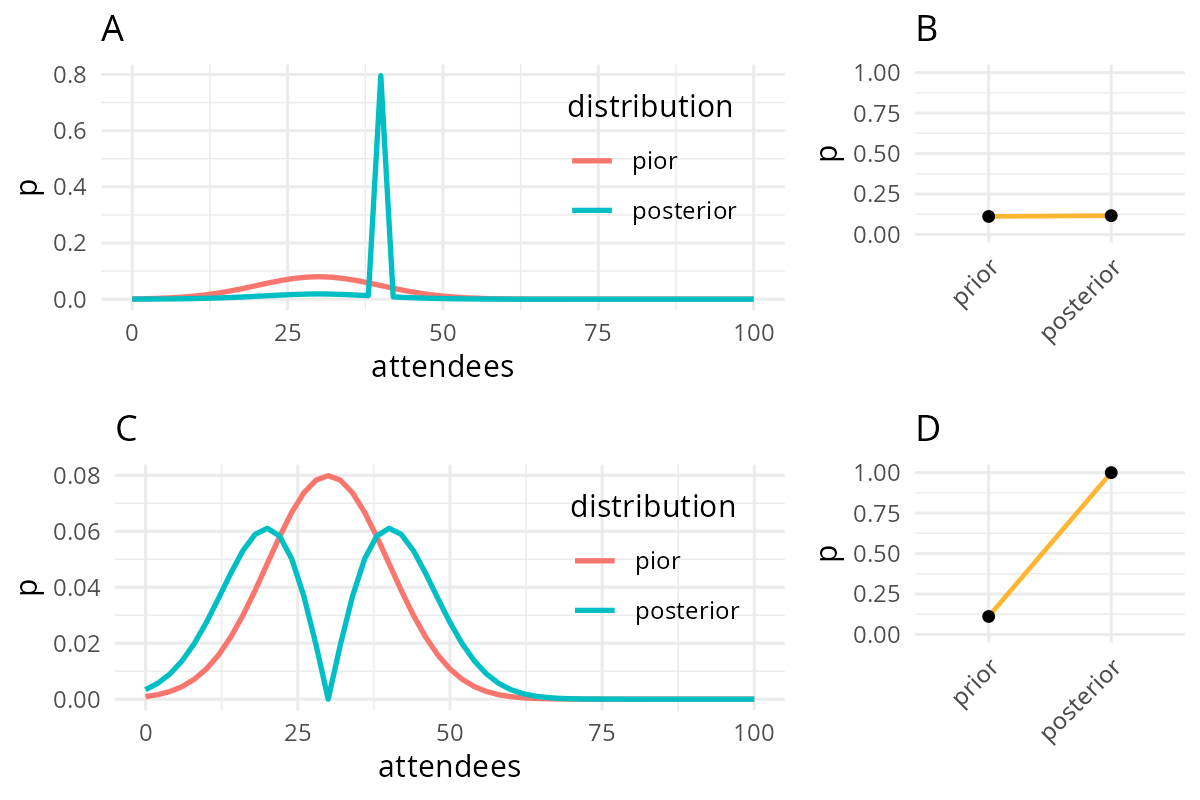
\includegraphics[width=\textwidth]{simplekao.png}\caption{Simulation of Kao et al.'s model applied to utterance \ref{e2} in Timid context. Plots A and C show the posterior distribution over the factual QUD for utterance ``{\em There were 40 people at the party}'' and ``{\em There were 100 people at the party}'', respectively. Plots B and D show the posterior probability of an affective interpretation for these utterances.}   \label{kao}
\end{figure}

Plots A and B in figure \ref{kao} show that utterances whose meaning is close to the norm are interpreted literally and don't have an impact on the affect prior. Plots C and D show that utterances whose meaning is far from the norm are not interpreted literally and change the affect prior entirely. This is all as it should be. A further prediction is made that hyperbolic utterances invite the inference that there is some deviation from the norm. The model doesn't predict, however, which direction that deviation should go into, which means that a hyperbolic utterance of \ref{e1} is not necessarily interpreted as many people turning up, but could potentially be seen as conveying that few (fewer than expected) people came. 

I believe the framework developed above may help to remedy these problems. In Kao et al.'s setup, as is standard in RSA, the prior and posterior distributions are distributions over a set of possibilities. No structure is assumed for this set. However, as we saw above, hyperbole is a phenomenon that depends on an ordering-induced QUD. What's more, given that hyperbole involves evaluation, we should take seriously the idea that interlocutors entertain aligment between the ordered partition related to the factual QUD and the scale of evaluation.  

To have a setup with two scales, we do the following. As before, we have a QUD that is a set of propositions and, as before, propositions can be ordered by some $\preceq$. We assume there is some scale of evaluation, an ordered set of degrees $\langle E,\leq\rangle$, and that propositions can be evaluated using a measure function $\epsilon: \wp(\mathcal{W})\rightarrow E$. 

The exact details of this measure function are unknown, but interlocutors may have simplifying assumptions that align $E$ and the QUD. (Think of things like: a party with more people is better than a party with fewer people, an accident with more casualties is worse than an accident with fewer, etc.) The simplest of such alignments would be the following:

$$s\preceq s'\ \Leftrightarrow \epsilon(s)\leq\epsilon(s')$$

In the original Kao et al. framework, there was a prior distribution $P$ over possibilities and for each possibility there was a probability of affect. Now, we have a scale of affect, or more accurately a scale of evaluation, which means that for each possibility we need a probability distribution over $E$. This distribution is informed by $\epsilon$. Obviously, $\epsilon(s)$ is the most likely evaluation of $s$. But there will be uncertainty as well, so we could take $\epsilon(s)$ as the mean of a normal distribution (with unknown standard deviation). Let $d$ range over degrees of evaluation ($d\in E$) and $s$ over cells in the factual QUD partition:

$$P(d|s) \sim \mathcal{N}(\mu=\epsilon(s),\sigma)$$


\begin{figure}[t]
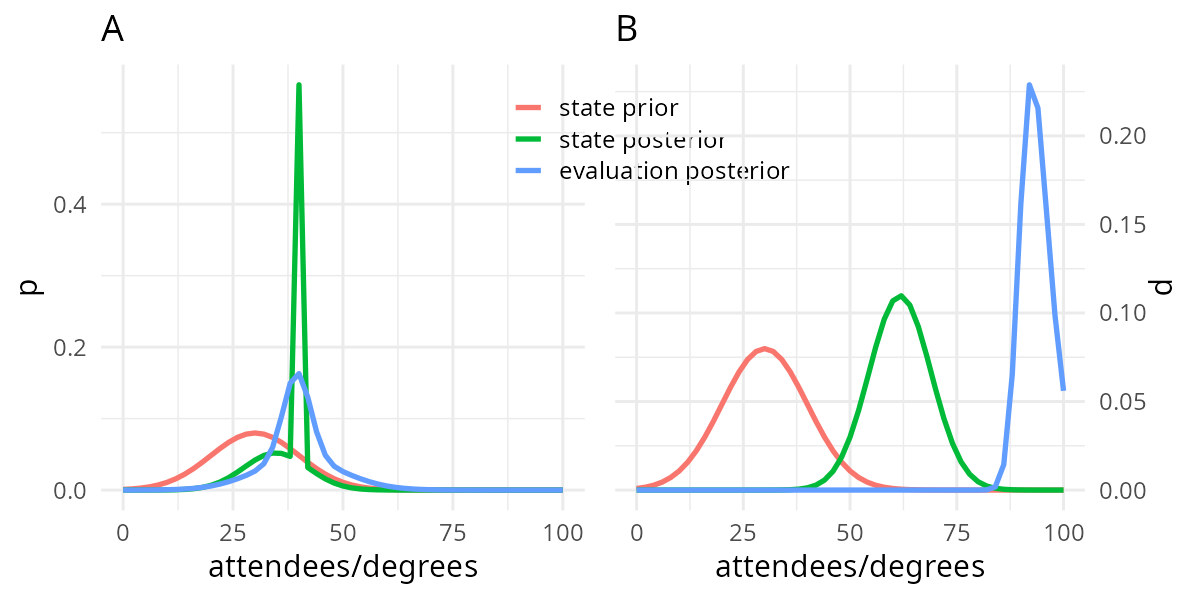
\includegraphics[width=\textwidth]{kaoalign.png}\caption{Simulation of the variation on the Kao et al.~model where scalar alignment is assumed between the order-induced factual QUD and the evaluation. The posteriors in plot A are for the utterance ``{\em There were 40 people at the party}'' and those in plot B are for ``{\em There were 100 people at the party}'.}\label{kaoa}
\end{figure}

Figure \ref{kaoa} shows the results from incorporating such a prior into a Kao et al. inspired RSA model. For the simulations $\epsilon$ aligned with the factual QUD. In fact, I represented the QUD as the set of integers \{0,\ldots,100\} and did the same for $E$. This allows confusion of representation of number of attendees and degrees of evaluation. So, for instance $\epsilon$({\bf 49}) = 49.   
Plots A and B show the prior distribution on the factual QUD, as well as posterior distributions for both states (factual QUD) and evaluation (affective/evaluative QUD). So, the x-axis in figure \ref{kaoa} plays a double role. From left to right the number of attendees increases, but so does the positivity of the evaluation.

Figure \ref{kaoa} shows that the alignment of evaluation and QUD changes the predictions made by the model. In plot A we see that utterances that express meanings close to normality are interpreted literally and that their evaluative meaning is moderate. Plot B shows that utterances whose literal meaning is extreme are not interpreted literally. They convey meanings that are in between the norm and the literal meaning. At the same time, their evaluative meaning is one that {\em is} extreme. So the hyperbolic utterance are interpreted as conveying extreme evaluation while at the same time they signal the untruth of the sentence uttered.

Another way of looking at plot B is that it shows the interpretive side of the definition I gave for hyperbole in section 3. We now have a probabilistic norm, but clearly the interpretation of hyperbole illustrated here is such that $n\prec h\prec \tau(M)$ (with $M$ the uttered sentence).
  
It will remain to be seen how good the predictions of this model are in other contexts. The assumed monotonic alignment is not always the most natural one. Think for instance about an utterance about today's temperature. Generally, extreme temperatures, both very high ones and very low ones, are evaluated as bad, while medium temperatures are good.\footnote{See \citet{nouwengoldi} for how exactly this kind of alignment drives the interpretation of degree adverbs.} A consequence of that particular pattern of evaluation is that the evaluation of extremely cold temperatures is indistinguishable from the evaluation of extremely hot temperatures. In accordance, the model will not be able to draw the correct inferences. For instance, hyperbolic ``{\em It's absolutely freezing}'' would wrongly be predicted to be compatible with (relatively) cold and with (relatively) warm temperatures. In other words, the (over)simplification that scalar alignment is monotonic does a lot of heavy lifting in predictions such as those in figure \ref{kaoa}.

\section{Conclusion}
\label{sec:orgf60a56f}

In this short paper, I have proposed to approach over- and understatements from a scalar formal framework. This framework allows us to provide explicit definitions that determine which transparently false statements count as overstatement and which count as understatement. I've also proposed an empirical test to ground predictions made by these definitions. Ultimately, my hope is that a relatively simple framework like the above will allow further study of untrue utterance and connected phenomena, like irony, utilising the formal rigour that truth-conditional semantics brings along.
Furthermore, as I showed in the previous section, the framework I developed connects naturally to computational approaches to rhetorical pragmatics. I leave a more detailed investigation of this combination for further research.

\bibliography{nouwen.bib}

\bibliographystyle{chicago}
\end{document}
